\documentclass[conference]{IEEEtran}
\usepackage[utf8]{inputenc}
\usepackage[T1]{fontenc}
\usepackage[spanish,es-tabla]{babel}
\usepackage{amsmath,amssymb}
\usepackage{graphicx}
\usepackage{booktabs}
\usepackage{array}
\usepackage{tabularx}
\usepackage{float}
\usepackage{siunitx}
\usepackage{hyperref}

\sisetup{output-decimal-marker={.}}
\newcolumntype{L}{>{\raggedright\arraybackslash}X}
\newcolumntype{C}{>{\centering\arraybackslash}X}
\renewcommand{\arraystretch}{1.15}
\graphicspath{{../figuras/}}

\begin{document}

\title{Evaluación de desempeño del ESP32-C6\\como controlador para el PiL de MARLUP}

\author{
\IEEEauthorblockN{Aarón Salas Alvarado, Mónica Solís Murillo, Eduardo Valle Arriola}
\IEEEauthorblockA{Instituto Tecnológico de Costa Rica}
}

\maketitle

\begin{abstract}
Se evaluó un ESP32-C6 (RISC-V de un núcleo a \SI{160}{MHz}, sin unidad de punto flotante) como posible controlador del lazo de posición de MARLUP. Un firmware de prueba midió, con el contador de ciclos del CPU, la aritmética básica, la duración de un paso del controlador PI del proyecto, el lazo periódico a frecuencias de \SI{1}{kHz} a \SI{1}{MHz}, la velocidad del ADC y el tiempo de ida y vuelta de una trama de seis bytes por USB. Un paso del PI tarda \SI{2.66}{\micro s} en \texttt{float} y \SI{4.51}{\micro s} en \texttt{double}; a los \SI{100}{Hz} de MARLUP ocupa el \SI{0.027}{\percent} del periodo. El lazo con el PI en \texttt{float} se sostiene sin plazos perdidos hasta \SI{200}{kHz}, pero al incluir la lectura del ADC el tope baja a unos \SI{25}{kHz}, porque cada lectura tarda \SI{36.7}{\micro s}. El tiempo de ida y vuelta por USB es de \SI{0.156}{ms} en promedio, muy por debajo del periodo de \SI{10}{ms}. El microcontrolador tiene capacidad de sobra para el lazo de MARLUP; su limitación práctica es que el flujo PIL de Simulink no lo soporta.
\end{abstract}

\begin{IEEEkeywords}
ESP32-C6, benchmark, microcontrolador, tiempo real, Processor-in-the-Loop.
\end{IEEEkeywords}

\section{Introducción}
El PiL de MARLUP se validó con un Arduino UNO R3 (ATmega328P, 8 bits, \SI{16}{MHz}). Para trabajos posteriores, como un PiL en tiempo real o el control de las tres patas, interesa saber si un microcontrolador más capaz y compacto, el ESP32-C6, tiene margen suficiente. Este reporte mide su desempeño en las operaciones que importan para el lazo: aritmética de punto flotante, el propio controlador PI, la ejecución periódica, la lectura del ADC y la comunicación con la PC.

\section{Hardware y método}

\subsection{Microcontrolador}
Los datos del chip se leyeron con \texttt{esptool} 5.6.0 (Tabla~\ref{tab:chip}). Se trata de un ESP32-C6FH4 con la memoria flash integrada en el encapsulado, lo que permite placas muy pequeñas. El núcleo RISC-V no tiene unidad de punto flotante, por lo que las operaciones con \texttt{float} y \texttt{double} se resuelven por software.

\begin{table}[H]
\centering
\caption{Datos del chip leídos con \texttt{esptool}}
\label{tab:chip}
\small
\begin{tabularx}{\columnwidth}{lL}
\toprule
Dato & Valor \\
\midrule
Chip & ESP32-C6FH4 (QFN32), revisión v0.1 \\
CPU & RISC-V, un núcleo a \SI{160}{MHz} + núcleo de bajo consumo \\
Memoria flash & \SI{4}{MB}, integrada en el chip \\
Cristal & \SI{40}{MHz} \\
Radio & Wi-Fi 6, Bluetooth 5 (LE), IEEE 802.15.4 \\
USB & USB-Serial/JTAG nativo \\
\bottomrule
\end{tabularx}
\end{table}

\subsection{Firmware y medición}
El firmware se compiló con el core de Arduino para ESP32 3.3.12 (placa \textit{ESP32C6 Dev Module}, \SI{160}{MHz}, \textit{USB CDC On Boot} activado). Todos los tiempos se miden con el contador de ciclos del CPU, cuya resolución es de \SI{6.25}{ns} a \SI{160}{MHz}. El controlador evaluado es el PI del proyecto: forma posicional con integral por Tustin, $K_p=60$, $K_i=1$, $T_s=\SI{10}{ms}$, saturación en $\pm1$ y anti-windup por \textit{clamping}, en versiones \texttt{float} y \texttt{double}. Un script de Python en la PC envía cada prueba por el puerto serie, recibe los resultados en CSV y genera las figuras. Las cinco pruebas son:
\begin{itemize}
\item \textbf{Aritmética}: lazos de $10^5$ a $10^6$ iteraciones de multiplicación y suma, división y raíz cuadrada.
\item \textbf{Paso del PI}: duración de 2000 pasos con entradas que imitan un escalón, descontando el costo de leer el contador.
\item \textbf{Lazo periódico}: el PI se ejecuta en cada instante programado, de \SI{1}{kHz} a \SI{1}{MHz}, durante unos \SI{0.5}{s} (hasta 20\,000 periodos), y se registra el retraso de cada inicio respecto al instante ideal. Se prueba el PI en \texttt{float}, en \texttt{double} y el PI en \texttt{float} precedido de una lectura del ADC. Si un inicio se retrasa más de un periodo, se cuenta como plazo perdido y el lazo se re-sincroniza.
\item \textbf{ADC}: 5000 lecturas consecutivas con \texttt{analogRead} a 12 bits.
\item \textbf{Comunicación}: 2000 tramas de seis bytes, con el mismo formato del PiL, enviadas desde la PC; el ESP32-C6 calcula el PI y responde seis bytes. La PC mide el tiempo de ida y vuelta (RTT).
\end{itemize}
El benchmark completo se corrió dos veces; la aritmética y las medianas del PI coincidieron. Se reportan los datos de la segunda corrida.

\section{Resultados}

\subsection{Aritmética}
La Tabla~\ref{tab:arit} y la Fig.~\ref{fig:arit} muestran el costo de no tener unidad de punto flotante. Una multiplicación y suma entera tarda \SI{25}{ns}, unos cuatro ciclos con la sobrecarga del lazo, mientras que en \texttt{float} tarda \SI{533}{ns}, unas 21 veces más, y en \texttt{double}, \SI{1160}{ns}. La división y la raíz cuadrada son todavía más costosas.

\begin{table}[H]
\centering
\caption{Aritmética a \SI{160}{MHz}}
\label{tab:arit}
\small
\begin{tabularx}{\columnwidth}{lCC}
\toprule
Operación & ns por operación & Millones de op./s \\
\midrule
\texttt{int32} mult. + suma & 25.2 & 39.7 \\
\texttt{float} mult. + suma & 533.5 & 1.87 \\
\texttt{double} mult. + suma & 1159.6 & 0.86 \\
\texttt{float} división & 793.1 & 1.26 \\
\texttt{double} división & 2650.0 & 0.38 \\
\texttt{sqrtf} & 4596.4 & 0.22 \\
\bottomrule
\end{tabularx}
\end{table}

\begin{figure}[H]
\centering
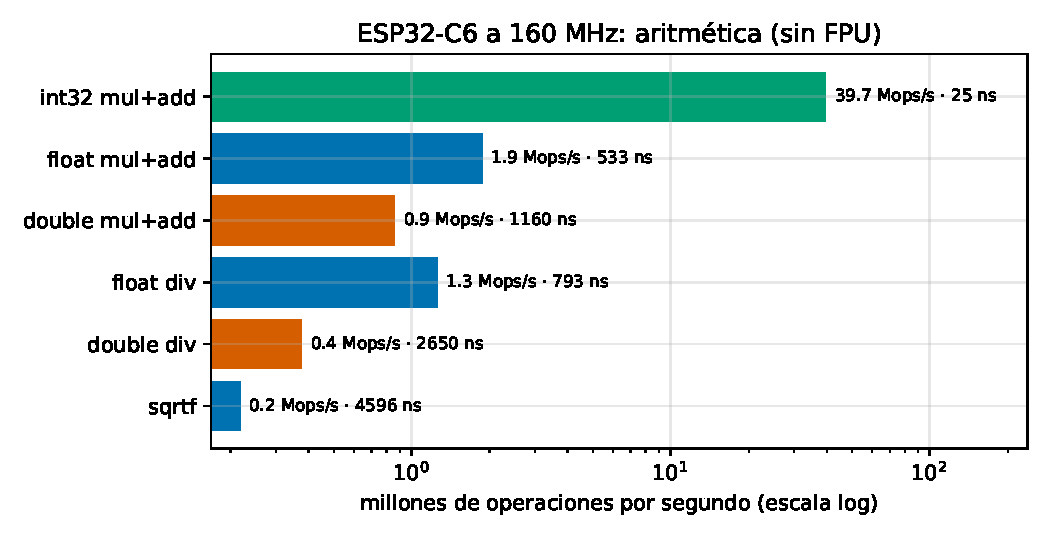
\includegraphics[width=\columnwidth]{1_aritmetica.pdf}
\caption{Rendimiento aritmético en escala logarítmica: enteros frente a punto flotante por software.}
\label{fig:arit}
\end{figure}

\subsection{Paso del controlador PI}
Un paso del PI tarda \SI{2.66}{\micro s} en \texttt{float} (426 ciclos, mediana) y \SI{4.51}{\micro s} en \texttt{double} (721 ciclos), como muestran la Tabla~\ref{tab:pi} y la Fig.~\ref{fig:pi}. Los máximos, de unos \SI{16}{\micro s}, corresponden a pocas muestras interrumpidas por el sistema operativo. Con la mediana, el tope teórico del lazo sería de \SI{376}{kHz} en \texttt{float} y \SI{222}{kHz} en \texttt{double}. A los \SI{100}{Hz} de MARLUP, el PI en \texttt{float} ocupa el \SI{0.027}{\percent} del periodo de \SI{10}{ms}.

\begin{table}[H]
\centering
\caption{Duración de un paso del PI (2000 pasos)}
\label{tab:pi}
\small
\begin{tabularx}{\columnwidth}{lCCC}
\toprule
Versión & Mediana (\si{\micro s}) & p99 (\si{\micro s}) & Máx. (\si{\micro s}) \\
\midrule
\texttt{float} & 2.66 & 2.81 & 16.29 \\
\texttt{double} & 4.51 & 12.67 & 15.66 \\
\bottomrule
\end{tabularx}
\end{table}

\begin{figure}[H]
\centering
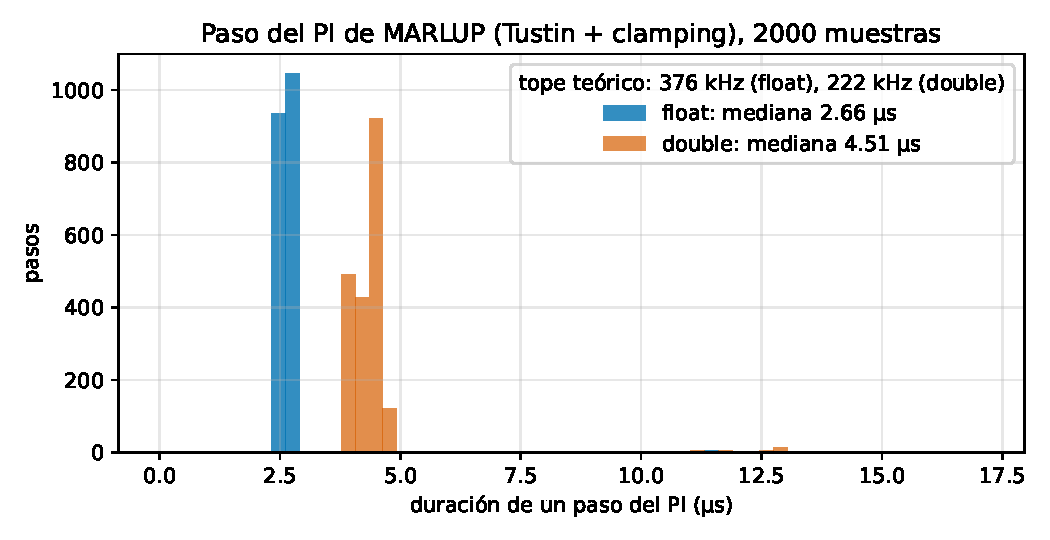
\includegraphics[width=\columnwidth]{2_paso_pi.pdf}
\caption{Distribución de la duración de un paso del PI de MARLUP.}
\label{fig:pi}
\end{figure}

\subsection{Lazo periódico en tiempo real}
La Fig.~\ref{fig:lazo} y la Tabla~\ref{tab:lazo} resumen hasta dónde se sostiene el lazo. Con el PI en \texttt{float} no se pierde ningún plazo hasta \SI{200}{kHz}, y la frecuencia lograda se satura en unos \SI{296}{kHz}. Con \texttt{double}, el lazo se sostiene hasta \SI{100}{kHz} y se satura en unos \SI{198}{kHz}. Al agregar la lectura del ADC, el límite baja a \SI{20}{kHz} sin pérdidas y a unos \SI{25}{kHz} como máximo. Mientras el lazo se sostiene, el retraso típico de cada inicio es de \SI{0.037}{\micro s}, del orden de la resolución de la medición, y el percentil 99 no pasa de \SI{6.3}{\micro s}. Por encima del tope, el porcentaje de plazos perdidos se estabiliza cerca del \SI{50}{\percent}: es un efecto del método, porque tras cada pérdida el lazo se re-sincroniza y el periodo siguiente vuelve a empezar a tiempo. Por eso la frecuencia lograda es la medida más representativa del límite.

\begin{table}[H]
\centering
\caption{Límites del lazo periódico}
\label{tab:lazo}
\small
\begin{tabularx}{\columnwidth}{lCC}
\toprule
Variante & Sin plazos perdidos hasta & Frecuencia lograda máx. \\
\midrule
PI \texttt{float} & \SI{200}{kHz} & \SI{296}{kHz} \\
PI \texttt{double} & \SI{100}{kHz} & \SI{198}{kHz} \\
ADC + PI \texttt{float} & \SI{20}{kHz} & \SI{25}{kHz} \\
\bottomrule
\end{tabularx}
\end{table}

\begin{figure*}[t]
\centering
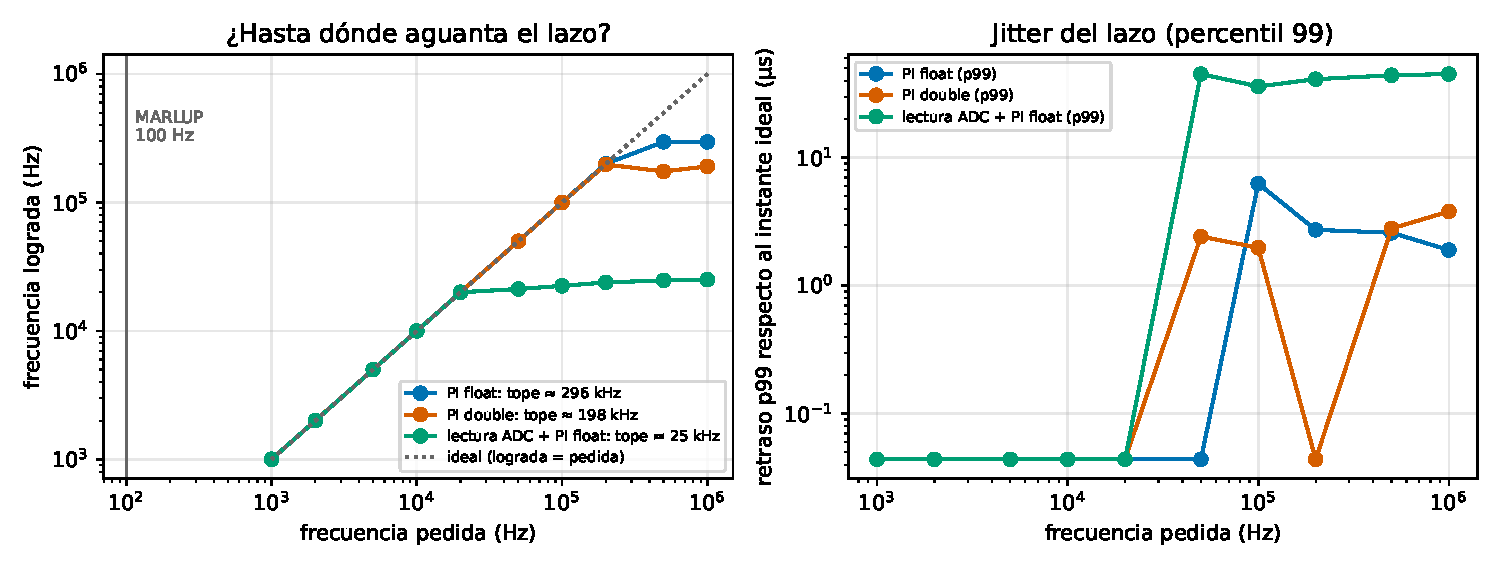
\includegraphics[width=0.9\textwidth]{3_lazo_tiempo_real.pdf}
\caption{Lazo periódico: frecuencia lograda frente a la pedida (izquierda) y retraso del percentil 99 respecto al instante ideal (derecha). La línea vertical marca los \SI{100}{Hz} de MARLUP.}
\label{fig:lazo}
\end{figure*}

\subsection{ADC}
Cada lectura con \texttt{analogRead} tarda \SI{36.7}{\micro s}, es decir, unas \num{27200} lecturas por segundo. Este es el cuello de botella del lazo con medición. La prueba se hizo con el pin sin conectar, por lo que solo es válida la velocidad; el ruido y la linealidad del ADC requieren una señal de referencia y no se evaluaron.

\subsection{Comunicación con la PC}
En las 2000 tramas, el tiempo de ida y vuelta fue de \SI{0.156}{ms} en promedio (\SI{0.135}{ms} de mediana), con percentil 95 de \SI{0.216}{ms}, percentil 99 de \SI{0.762}{ms} y máximo de \SI{3.22}{ms} (Fig.~\ref{fig:rtt}). Solo 2 tramas superaron \SI{1}{ms} y ninguna se acercó al periodo de muestreo de \SI{10}{ms}. El valor incluye la sobrecarga del lado de la PC (Windows y Python), así que la latencia propia del enlace USB es menor.

\begin{figure}[H]
\centering
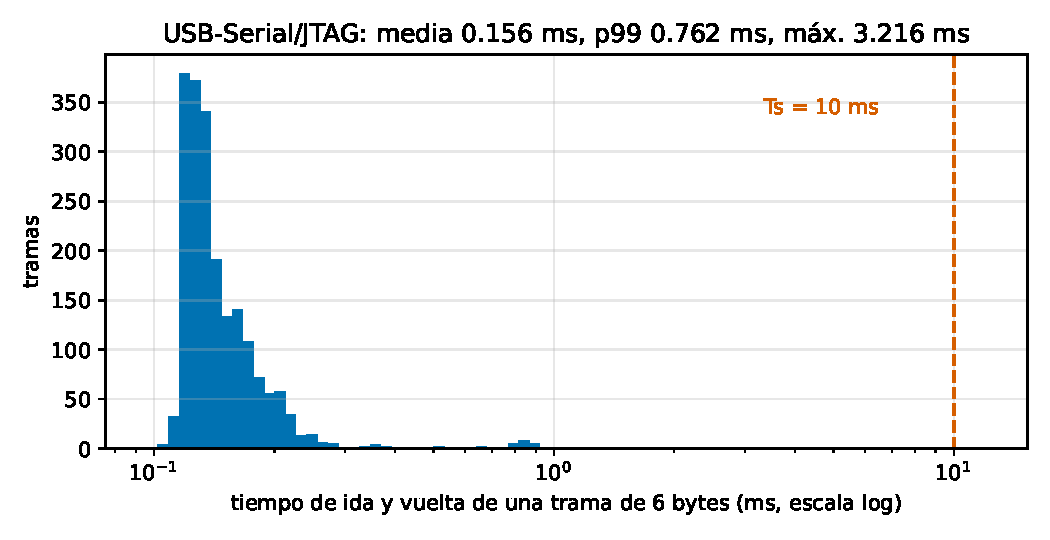
\includegraphics[width=\columnwidth]{4_rtt_usb.pdf}
\caption{Tiempo de ida y vuelta de una trama de seis bytes por USB-Serial/JTAG (escala logarítmica).}
\label{fig:rtt}
\end{figure}

\section{Discusión}
Para MARLUP, que muestrea a \SI{100}{Hz}, el ESP32-C6 tiene un margen muy amplio: el PI ocupa una fracción mínima del periodo y el lazo completo con lectura del ADC podría correr unas 200 veces más rápido. Tres observaciones guían su uso. Primero, conviene implementar el controlador en \texttt{float}, porque sin unidad de punto flotante \texttt{double} cuesta cerca del doble. Segundo, el límite práctico lo impone el ADC y no el cómputo; si se necesitara más velocidad, habría que usar el modo continuo del ADC en lugar de lecturas individuales. Tercero, la comunicación USB es lo bastante rápida y estable para un PiL en tiempo real. Su mayor limitación para el curso no es de desempeño: el \textit{Simulink Support Package for Arduino Hardware} instalado (R2026a) no incluye el ESP32-C6, y sus placas ESP32 no ofrecen el modo PIL, por lo que un PiL con este chip requeriría un protocolo de comunicación propio.

\section{Conclusiones}
\begin{itemize}
\item Un paso del PI de MARLUP tarda \SI{2.66}{\micro s} en \texttt{float} y \SI{4.51}{\micro s} en \texttt{double}; a \SI{100}{Hz} ocupa el \SI{0.027}{\percent} del periodo.
\item El lazo con el PI en \texttt{float} se sostiene sin plazos perdidos hasta \SI{200}{kHz}; con lectura del ADC, hasta \SI{20}{kHz}, limitado por los \SI{36.7}{\micro s} de cada lectura.
\item Sin unidad de punto flotante, las operaciones \texttt{float} cuestan unas 21 veces más que las enteras y las \texttt{double}, el doble que las \texttt{float}.
\item La comunicación por USB tiene un tiempo de ida y vuelta medio de \SI{0.156}{ms} y máximo de \SI{3.22}{ms}, muy por debajo del periodo de \SI{10}{ms}.
\end{itemize}
Como trabajo futuro se propone medir el ruido y la linealidad del ADC con una señal de referencia, correr el mismo benchmark en el Arduino UNO para una comparación directa, e implementar un PiL en tiempo real con el ESP32-C6 marcando su propio periodo de muestreo.

\appendix
\section*{Anexo: reproducibilidad}
Repositorio: \url{https://github.com/aasalas/LAB-DE-CONTROL-GR5}, carpeta \texttt{EXPERIMENTOS/esp32c6\_benchmark}: firmware en \texttt{esp32c6\_benchmark/}, script \texttt{correr\_benchmark.py} (se ejecuta con \texttt{python correr\_benchmark.py COM7}), datos en \texttt{resultados/} y figuras en \texttt{figuras/}.

\end{document}
